%%%%%%%%%%%%Outline%%%%%%%%%%%%%%%%%%

%%%
% message<introduction to this section>
% opening sentence
% ref to each subsection

%%% subsection 4.1 <Hardware Specialization via Kinsn-based Bytecode Transformations>

%%%
% message<kinsn is a dedicated instruction form in eBPF bytecode>
% first-class instruction site in the program
% explicit optimization intent retained in bytecode
% encoded as a sidecar plus a kinsn call
% ordinary eBPF only appears as instantiated form for checking or fallback

%%%
% message<kinsn representation makes optimization intent explicit in bytecode>
% two components:
%  - target / instruction family
%  - sidecar / operand-binding payload
% sidecar carries regs, immediates, mode bits
% concrete running example: select64
% why target + sidecar better than later JIT pattern recovery

%%%
% message<each kinsn has one canonical semantics shared by verifier and JIT>
% module descriptor defines the canonical instantiated ordinary-BPF sequence
% the same descriptor may also provide architecture-specific native emission
% one instruction contract shared across verification and execution

%%%
% message<the verifier checks kinsn by temporarily lowering it to ordinary eBPF>
% replace each kinsn with its instantiated proof sequence
% run the standard verifier on the lowered program
% restore the original kinsn encoding after verification
% ordinary eBPF serves as the proof form

%%%
% message<the JIT uses the original kinsn representation for direct native lowering>
% keep the original kinsn until code generation
% dispatch on target and payload to emit native code
% avoid recovering lost intent from flattened ordinary BPF
% rewrite to the same instantiated ordinary-BPF sequence when native emit is unavailable
% native lowering must preserve the canonical kinsn semantics

%%% subsection 4.2 <Runtime Specialization via Deployment-time Bytecode Transformations>

%%%
% message<xx>
% xx

%%%%%%%%%%%%Outline%%%%%%%%%%%%%%%%%%


\section{Bytecode-Level Optimization}
\label{sec:bytecode}

This section introduces \emph{kinsn}, a bytecode abstraction that separates the representation used to preserve optimization intent from the ordinary-eBPF form used for kernel verification. A kinsn keeps operations such as \texttt{rotate64}, \texttt{select64}, and \texttt{extract64} explicit in the bytecode, instead of forcing the compiler to flatten them early into ordinary-eBPF idioms. For verification, each kinsn is expanded into a semantics-equivalent ordinary-eBPF sequence and checked by the kernel's existing verifier. For execution, the original kinsn is lowered directly to target code while its higher-level semantics remain explicit. This separation keeps sophisticated optimization in userspace, preserves the current kernel verification interface, and avoids pushing target-specific recovery logic into the in-kernel JIT.

We first describe how a kinsn is represented in extended eBPF bytecode (§\ref{subsec:kinsn-repr}). We then explain how the same kinsn is interpreted by verification and execution (§\ref{subsec:kinsn-semantics}). The key point is that these two paths implement the same instruction contract: verification reasons about the instantiated ordinary-eBPF sequence, while JIT code generation may directly emit architecture-specific instructions from the original kinsn representation. §\ref{sec:rejit} then shows how BPFreJIT constructs and uses kinsns in its rewrite pipeline.

\begin{table}[t]
\centering
\small
\setlength{\tabcolsep}{4pt}
\begin{tabular}{p{0.34\columnwidth} p{0.26\columnwidth} p{0.26\columnwidth}}
\toprule
\textbf{Kinsn} & \textbf{x86} & \textbf{ARM64} \\
\midrule
\texttt{rotate64} & \texttt{ROL}/\texttt{ROR} & \texttt{EXTR} \\
\texttt{select64} & \texttt{CMOV} & \texttt{CSEL} \\
\texttt{extract64} & \texttt{BEXTR} & \texttt{UBFM} \\
\texttt{endian\_load64} & \texttt{MOVBE} & \texttt{REV} \\
\texttt{speculation\_barrier} & \texttt{LFENCE} & \texttt{DSB SY + ISB} \\
\bottomrule
\end{tabular}
\caption{Currently implemented kinsn targets and their x86/ARM64 native lowerings.}
\label{tab:kinsn-implemented}
\end{table}


\subsection{Representation of Kinsn}
\label{subsec:kinsn-repr}

Kinsn is a dedicated instruction form in eBPF bytecode. A program may therefore contain explicit kinsns, rather than encoding every optimization opportunity as an ordinary-BPF instruction sequence. This design keeps optimization intent in the bytecode itself, where later compilation stages can still observe and exploit it. Concretely, each kinsn is encoded as a sidecar plus a kinsn call. Ordinary eBPF appears only as an instantiated form: it is used when the kernel needs a verifier-visible proof sequence and when a kinsn must fall back to the generic path.

% [addressed] \note{hao: We have a mismatch here. The text says sidecar, but the figure uses 'binding'.}

\begin{figure*}[htbp]
  \centering
  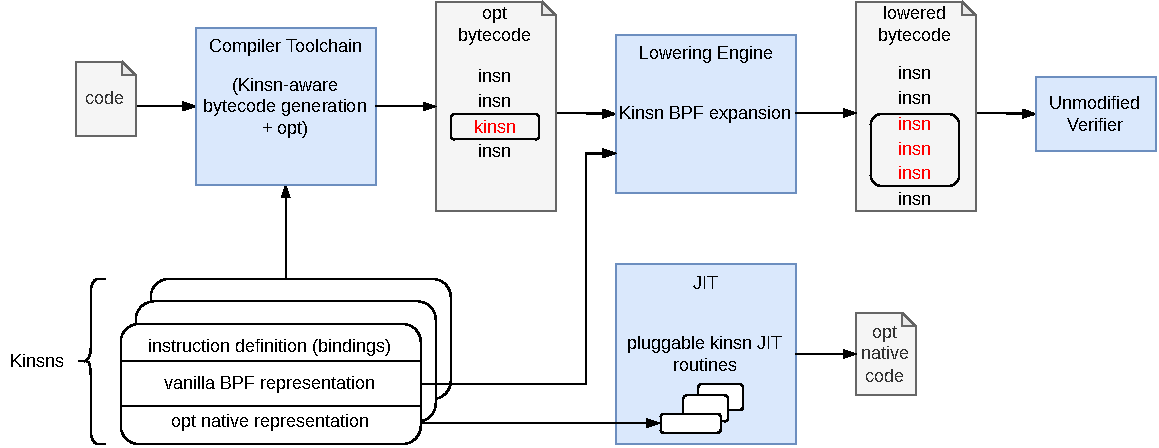
\includegraphics[width=0.92\textwidth]{figures/sec-3-flow.drawio.pdf}
  \caption{BPF Optimization Pipeline utilizing specialized Kernel Instructions (Kinsns).}
  \label{fig:kinsns-opt}
\end{figure*}


Each kinsn is represented by two parts: a \emph{target} and a \emph{sidecar} payload. The target identifies the instruction family, such as \texttt{rotate64}, \texttt{select64}, \texttt{extract64}, or an endian-aware load. The sidecar binds that abstract operation to a concrete program point by encoding the relevant registers, immediate fields, and mode bits. Figure~\ref{fig:select64-kinsn} uses \texttt{select64} as a running example. In ordinary eBPF, the operation appears as a small branch diamond. In kinsn form, the same operation appears as one instruction kinsn whose target names the operation and whose sidecar carries the destination register, the condition input, and the candidate values. This split is important because it preserves the semantic structure that later lowering wants to realize directly, instead of forcing the JIT to recover that structure from already flattened ordinary-BPF code.

% [] \note{hao: instead of a new subsection, does it make sense to explain kinsn from: (1) how compilers can use it, and what is the benefit? (2) the verifier's behaviour, (3) the JIT's behaviour. And finally, safety guarantee. }
\subsection{Kinsn Semantics in Verification and Execution}
\label{subsec:kinsn-semantics}

Each kinsn has one canonical semantics shared by the verifier and the JIT. A module-side descriptor defines how the kinsn is instantiated into an equivalent ordinary-BPF sequence, and it may also provide architecture-specific native emission routines for direct lowering. The instantiated ordinary-BPF sequence is the canonical, verifier-visible meaning of the kinsn. Native lowering does not define a different meaning; it is another realization of the same instruction contract.

% [] \note{hao: why proof form? No proof here, just insns.}
The verifier checks kinsn by temporarily lowering each kinsn to its instantiated ordinary-BPF sequence. The kernel replaces the original kinsn with this proof sequence, runs the standard eBPF verifier on the lowered program, and then restores the original kinsn encoding after verification succeeds. In this design, ordinary eBPF serves as the proof form for kinsn. The verifier does not need to reason about target-specific machine code, and kinsn does not require a separate safety checker.

Execution follows a different path while preserving the same semantics. The original kinsn representation is kept until code generation, and the JIT backend dispatches on the target and sidecar payload to emit an architecture-specific native sequence directly from that representation. For example, the \texttt{select64} kinsn in Figure~\ref{fig:select64-kinsn} can lower to a conditional-move sequence on x86 rather than re-materializing the branchy ordinary-BPF proof form. When direct native emission is unavailable for a kinsn, the kernel rewrites that kinsn to the same instantiated ordinary-BPF sequence used by the verifier and continues with the generic path. Thus, verification and execution follow different lowering paths, but both remain anchored to the same canonical kinsn semantics.

%[] \note{hao: here is a nice place to argue why we preserve the verifier's safety guarantee down to the native's execution. }
% TODO: \noindent\textbf{Kinsn Safety.} Define the equivalence between kinsn and native, assume the correctness of one-to-one mapping (the existing JIT), then by transitivity, the native is safe as the bytecode.
